%%%%% Document Setup %%%%%%%%

\documentclass[12pt, onecolumn]{revtex4}    % Font size (12pt) and column number (one or two).

\usepackage[a4paper, left=2.5cm, right=2.5cm, top=2.5cm, bottom=2.5cm]{geometry}  % Defines paper size and margin length

\renewcommand{\baselinestretch}{1}     % Defines the line spacing

\usepackage{subcaption}

\usepackage[font=small, labelfont=bf]{caption}                      % Defines caption font size and caption title bolded
\captionsetup[figure]{justification=justified, singlelinecheck, font=small} 
\captionsetup[table]{justification=justified, singlelinecheck=off, font=small} 
\captionsetup{compatibility=false}

\usepackage{graphics,graphicx,epsfig,ulem}	% Makes sure all graphics works
\usepackage{amsmath} 						% Adds mathematical features for equations

\usepackage{fancyhdr}

\usepackage{textcomp}

\usepackage{tabularx}

\def\thesection{\arabic{section}}
\def\thesubsection{\alph{subsection}}

\def\bibsection{\section*{References}}        % Position reference section correctly

%%%%% Document %%%%%
\begin{document}                     

\title{Testing the Milankovitch-Croll hypothesis using $\delta^{18}$O foram data} 
\maketitle
%\thispagestyle{plain} % produces page number for front page

\vspace{-4ex}

The Milankovitch-Croll hypothesis suggests that changes in the Earth's orbit around the Sun leads to fluctuations in solar insolation thus affecting Earth's planetary climate \cite{ruddiman_climate}. The hypothesis can be explored by analysing proxy data (deep ocean sediment cores) and Earth orbital data. Sediment cores provide a trace to measure the global temperature fluctuations and global ice volume across Earth's history, the $\delta^{18}$O ratio in foram shells \cite{droxler_climate}. \\

% cite the original Milankovitch paper for the reference on what the hypothesis is?

Defined from laboratory experiments, a $\sim 5^{\circ}\mathrm{C}$ temperature increase leads to an $\sim 1$\textperthousand\ decrease in the $\delta^{18}$O ratio. As ice-sheets melt, more $^{16}$O is released into the oceans, therefore reducing the ratio. Sediment core data for an early (0.0 to 1.0 Myr BP) and late (4.0 to 5.0 Myr BP) period of Earth's history (Fig.~\ref{fig:foram_data}) indicates that in the more recent age the temperature had been varying more dramatically in line with the amplitude of the $\delta^{18}$O. This would have lead to longer periods of cooling and with a cooler climate, there would have been a larger amount of global ice. In both sets of $\delta^{18}$O data, there features a sinusoidal-like trend. Whilst the older data has a smaller amplitude, it can still be suggested that the glacial-interglacial events are a normal part of Earth's planetary climate cycle and there could be an origin from the cyclical Earth-Sun orbit relationship. \\

In analysing the astrophysical data there are three concepts to consider: (i) eccentricity, (ii) precession, and (iii) obliquity. The former describes the ellipticity of the Earth's orbit around the Sun \cite{carroll_astro}, it's effect on insolation however is not entirely independent as the eccentricity depends on the orbital angle between the solstices and the position of perihelion/aphelion. A precessional index value can be produced with $\chi= \varepsilon \sin{\omega}$, where $\varepsilon$ is the eccentricity and $\omega$ is the angle. Finally the obliquity can be defined as the value which describes the degree of tilt of the Earth's axis relative to the orbital plane.  \\

To evaluate and verify that our orbital data agrees with literature, two statistical techniques can be applied. The first is \textit{wavelet transform} (WT) analysis, by using the WT tool in PAST3 \cite{past3} heatmaps (Fig.~\ref{fig:wa_orbital_data}) can be obtained which contain the dominant frequencies from a dataset. The second technique is \textit{REDFIT} analysis, frequencies (Fig.~\ref{fig:d18o_redfit}) can be picked out by finding peaks which have a height greater than a $95\%$ confidence interval. Processing the orbital data with these two tools results can be obtained (Table \ref{table:final_results}) which have an average $\sim 96 \%$ agreement when compared with literature wavelengths. Knowing that the methods are valid and that they produce accurate results, the $\delta^{18}$O foram data can be analysed with the same tools. \\

Initially looking at the data, there is a signal which could be attributed to the obliquity as there are wavelengths of 41.1 ka (REDFIT) and 38.9 ka (WT) which are comparable to the actual value of 41 ka. However from WT analysis (Fig.~\ref{fig:wa_d18o}) this obliquity is only prevalent from 0.15 Myr to 1.28 Myr BP. Beyond this there is a complete disconnect which could be attributed to the rise of eccentricity as the wavelengths are $\sim 100$ ka. Using WT, from $\sim 1.28$ Myr to 4.80 Myr BP there contains 96.0 ka, and similarly with REDFIT a wavelength of 96.3 ka can be found.  It is therefore not unreasonable to search for a third signal which can then be associated with the perihelion longitude. Consequently one signal is apparent, 23.7 ka, but it can only be seen with REDFIT analysis. The lack of this in WT could be attributed to the fact that the data is dominated and spanned by an ``extended eccentricity signal''. Before 1.28 Myr BP and after 4.80 Myr BP, there are additional wavelengths of 945.5 ka and 1247.6 ka. It could be suggested that the latter signal is related to the eccentricity as it is a multiple of the strongest yet missing component of eccentricity forcing \cite{berger_climate}, 413 ka. \\

Through an analysis of the $\delta^{18}$O data it can be implied that that the Milankovitch-Croll hypothesis does have some merit, however there are various issues and questions which prevent the theory from being fully accepted. \\

One prevailing issue is why do the orbital features in the benthic foram data not span the entirety of the data set? If the hypothesis was to be taken at face value then it would be expected that a signal should be seen across the WT analysis, as is seen for the individual analyses of the orbit data (Fig.~\ref{fig:wa_orbital_data}). \\

% However, if it is the most powerful, then why cannot it be detected throughout the data set? Why must it be in the form of a multiple?

% and even with the REDFIT fitting (Fig.~\ref{fig:d18o_redfit}) it can be seen that this perihelion signal is weak compared to the other two peaks. \\

\newpage

%\twocolumngrid

\bibliographystyle{unsrt}
\bibliography{practical_2}

\newpage

\section*{Appendices}
\begin{figure}[!h]
\begin{center}
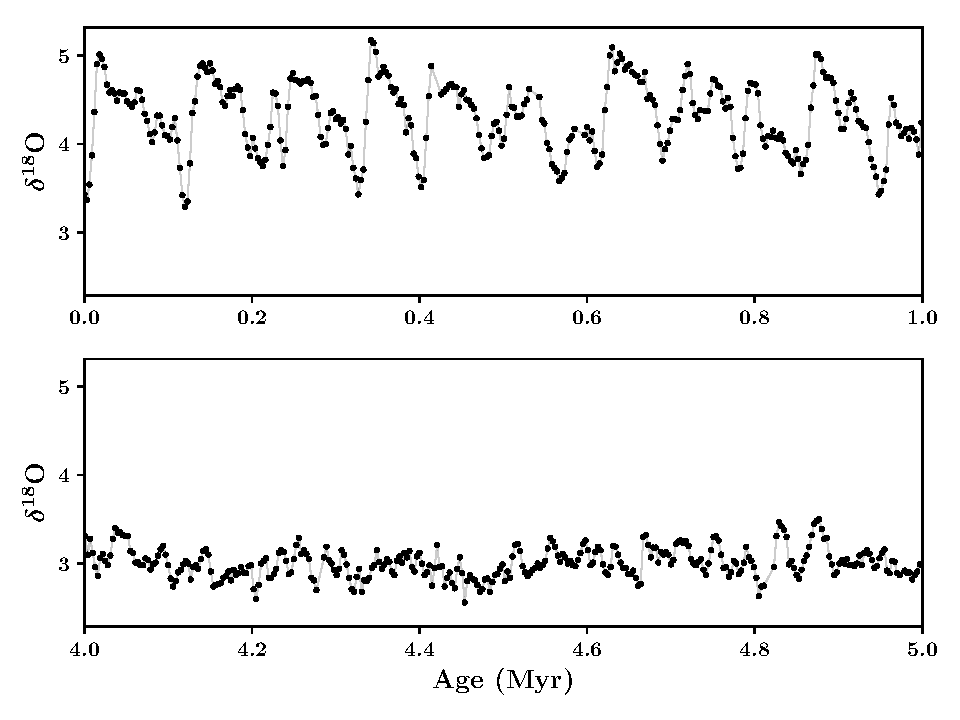
\includegraphics[width=11cm]{figures/foram_data}
\caption[]{Plots of the marine benthic foram $\delta^{18}$O data against age, with increasing time to the right. Both data sets have been taken out of a larger set which spans from 0 Myr to 6 Myr. As we move closer towards the present day, the periodicity and amplitude is larger which implies more extreme temperature variations so longer glacial-interglacials and a larger change in the global ice volume.}
\vspace{-3ex}
\label{fig:foram_data}
\end{center}
\end{figure}

\begin{figure}[!h]
\begin{center}
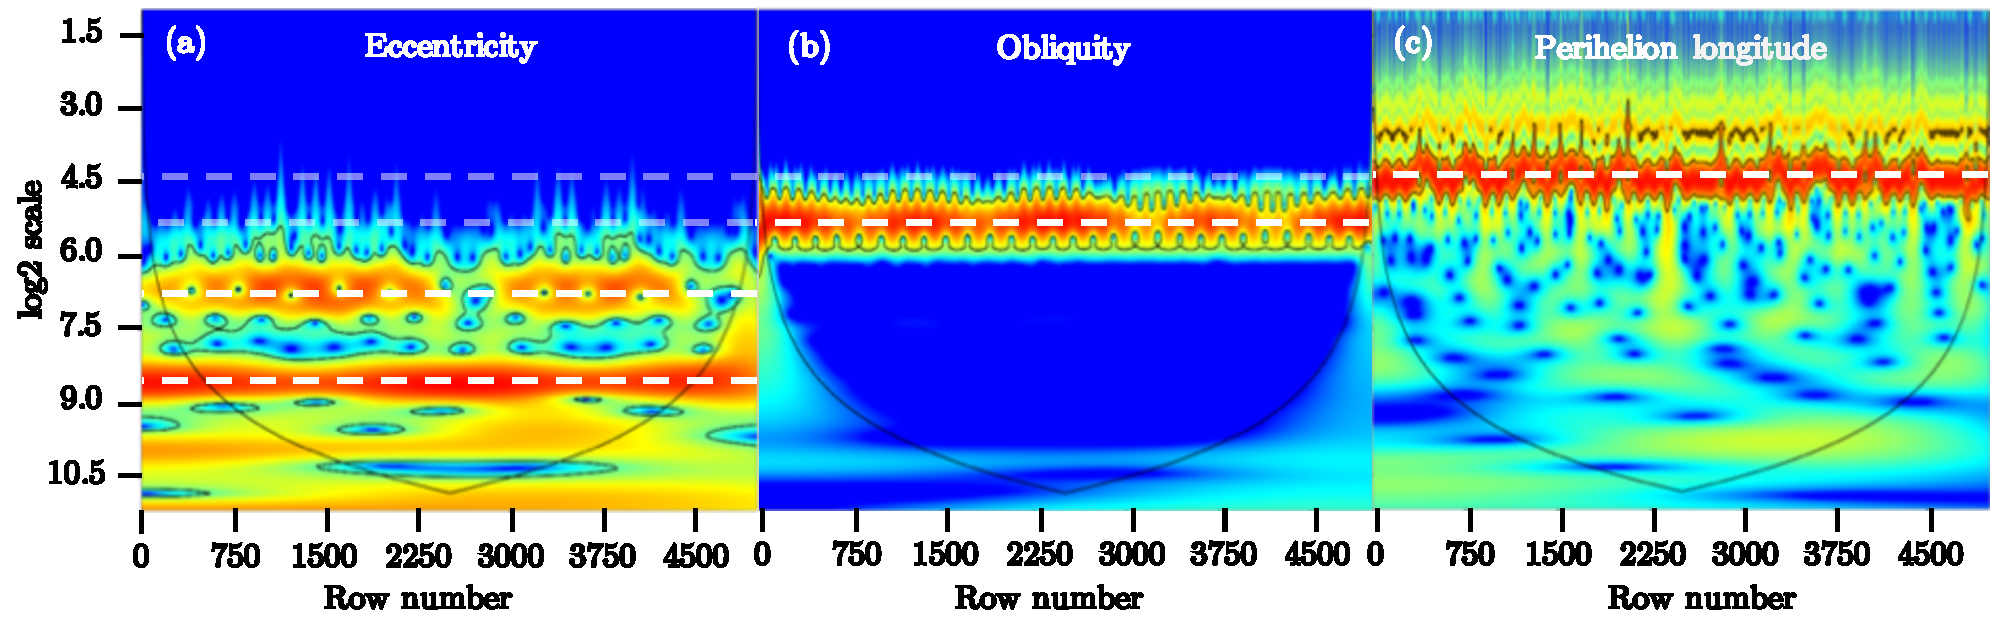
\includegraphics[width=16cm]{figures/wa_orbital_data}
\caption[]{The eccentricity, obliquity and perihelion longitude (precession) orbital data which has been processed with the wavelet transform analysis tool in PAST3. The periodicities from the data can be obtained by considering the ``hottest'' areas of each of the heat maps (i.e. the red/orange areas). Values for the wavelength can be found with $2^y \times P$, where $y$ is the y-axis height of the hot region, and $P$ is the period of time between the data points. In Table \ref{table:final_results} we summarise the wavelengths which correspond to the dashed-line heights.}
\vspace{-3ex}
\label{fig:wa_orbital_data}
\end{center}
\end{figure}

\begin{figure}[!h]
\begin{center}
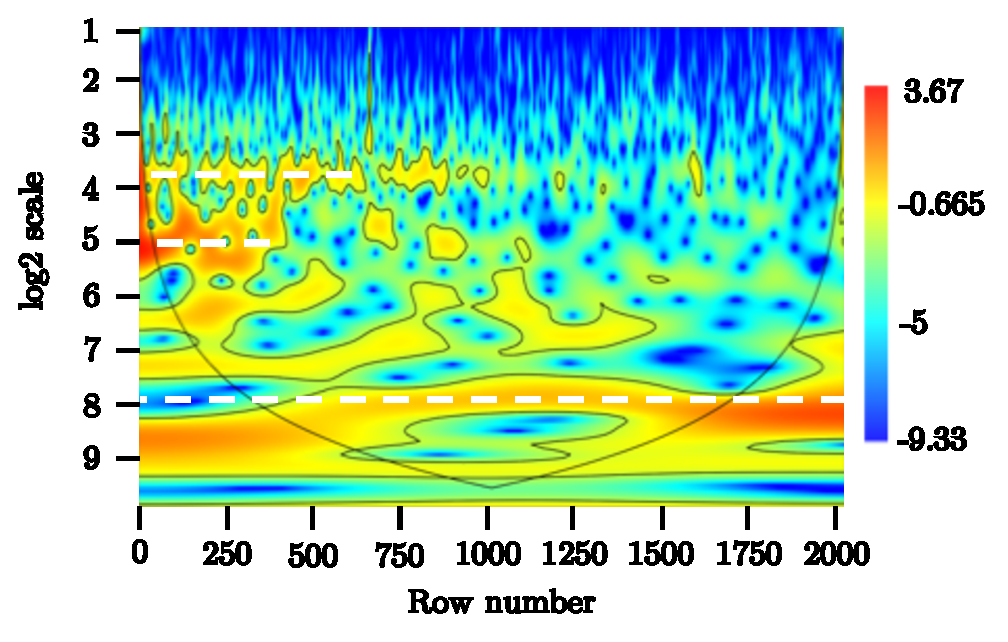
\includegraphics[width=11cm]{figures/wa_d18O.pdf}
\caption[]{The result from applying the PAST3 wavelet transform analysis tool to the $\delta^{18}$O benthic foram data, the wavelengths found are summarised in Table \ref{table:final_results}. The results are similar to those found in the orbital data, which could imply that orbital forcing does have an influence on glacial-interglacial climate.}
\vspace{-3ex}
\label{fig:wa_d18o}
\end{center}
\end{figure}

\begin{figure}[!h]
\begin{center}
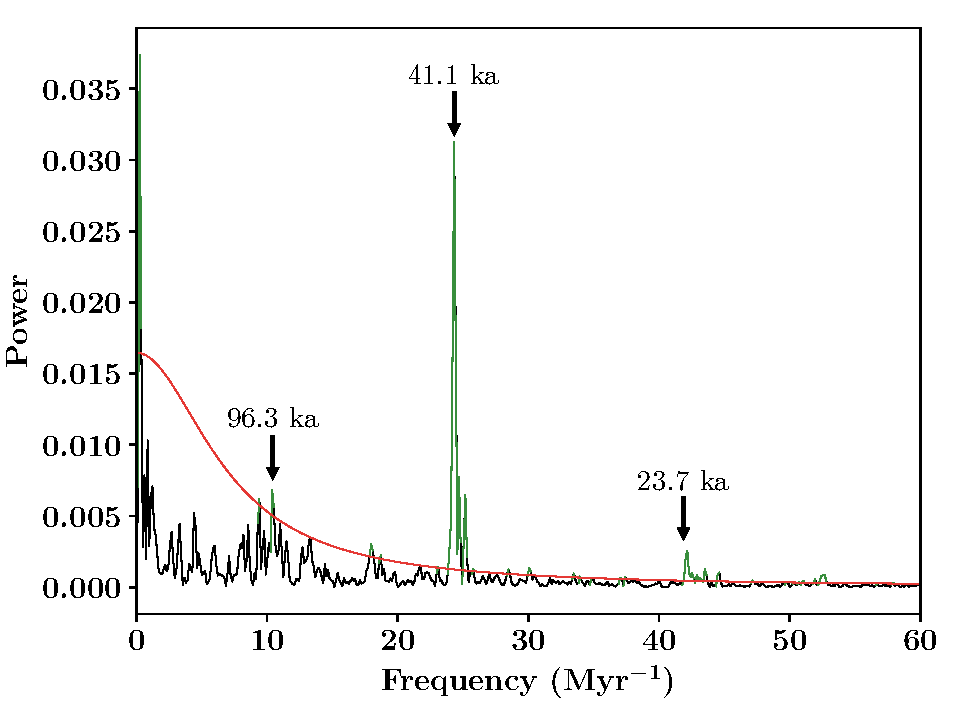
\includegraphics[width=11cm]{figures/d18O_redfit}
\caption[]{The benthic foram $\delta^{18}$O data analysed using the REDFIT spectral analysis tool in PAST3. Three dominant signals can be seen as coloured in green, they are defined as the main signals as they have a height greater than the $95\%$ confidence interval (the red curve). The same results can be found in Table \ref{table:final_results}, and comparing to the ``true'' wavelengths we also find similarities which further strengthens the possibility that the Milankovitch-Croll hypothesis has some validity.}
\vspace{-3ex}
\label{fig:d18o_redfit}
\end{center}
\end{figure}

\begin{table}[h!]
\centering
\begin{tabular}{c@{\hskip 20pt}c@{\hskip 20pt}c@{\hskip 20pt}c} 
 \hline
  & \textbf{Literature (ka)} &\textbf{REDFIT (ka)} & \textbf{WT (ka)} \\ [0.5ex] 
 Eccentricity & 100, 413 & 95.2, 128.2, 416.7 & 89.1, 100.4,  401.7\\
 Perihelion Longitude & 23, 100 & 23.8, 22.2 & 21.1 \\
 Obliquity & 41 & 41.7 & 39.4 \\
 $\delta^{18}$O & & 23.7, 41.1, 96.3  & 38.9, 96.0, 271.5, \\
 & & & 945.5, 1247.6 \\
 \hline
\end{tabular}
\caption{Table showing different sets of wavelength data: the approximate correct wavelengths for the periodicity of the orbital features \cite{campisano_milankovitch}, the results of the REDFIT spectral analysis and Wavelet Transform (WT) analysis on the orbital and benthic foram data. We find that as tools both REDFIT and WT are able to obtain similar periodicities which then agree with the literature values. }
\vspace{-0.5em}
\label{table:final_results}
\end{table}

\end{document}